\chapter{Theory}
\label{chap:theory}

% Überblick über die Idee schaffen -> Virtueller Speicher durch funktion möglich

% -------------------------------------------------------------------------------------------------
%                                            Idea
% -------------------------------------------------------------------------------------------------

\section{The Idea}
% Idea Description

% Steps necessary to implement Idea

% Gegenüberstellung: Normaler HW Page Table Walk - Mapping function

% Normal Page Table Walk
\begin{figure*}[ht!]
    \centering
    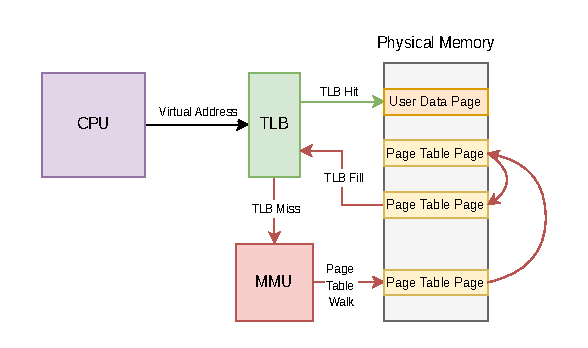
\includegraphics[scale=1.5]{figures/theory_normal_tlb_miss.pdf}
    \caption[Usual TLB Miss]{This figure shows what usually happens when the TLB misses:
        the miss will invoke the hardware state machine page table tree walker; the walker traverses
        the page table tree and if a valid PTE is found, the mapping is added to the TLB. The processor
        then executes the failing instruction again which will then result in a TLB hit}
    \label{fig:theory:normal_tlb_miss}
\end{figure*}

% TODO der Zwischenschritt mit dem Software Page Table walk wird dann in der Impl
% eingeführt

% Virtual Memory using a Mapping Function
\begin{figure*}[ht!]
    \centering
    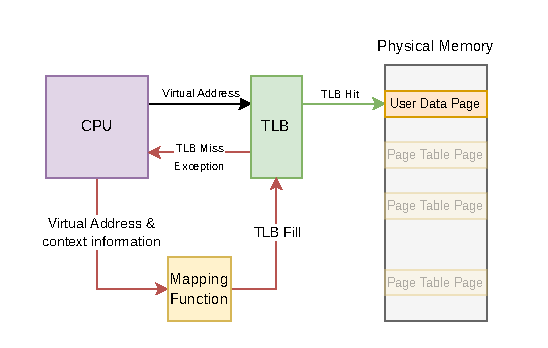
\includegraphics[scale=1.5]{figures/theory_mapping_fx.pdf}
    \caption[Virtual Memory using a mapping function]{Instead of emulating a hardware page table walk in software on
        a TLB Miss exception, a mapping function is invoked that calculates the PTE using arithmetic primitives and tries
        to avoid memory references.}
    \label{fig:theory:mapping_fx}
\end{figure*}





% The Idea -> Getting rid of any memory access in favor of simple arithmetic operation (eg. hash functions)
Die grundlegende Idee dieser Arbeit ist es die Page Table Strukturen, seien es Hashed Page Tables oder
Radix Page Tables, oder andere Designs wie sie in Related work presentiert wurden, komplett loszuwerden.
Diese sollen durch eine einfache funktion ersetzt werden die das Mapping von virtuellen zu physischen
Addressen realisiert.\\
Offensichtliche Kandidaten für so eine Funktion wären natürlich Hashfunktionen. Vor allem die in
\cite{skarlatos2020elastic} vorgestellte Elastic Cuckoo Hash function verfügt schon über Eigenschaften
die für ein direktes virtual-physical mapping, statt einem virtual-hash table index, nützlich wären.
\todo{Das mit den Cuckoo hash ist vielleicht für diese Stelle schon zu viel detail}.
Der wichtigste Aspekt diese Funktion ist allerdings, dass sie, anders als alle anderen Page Table designs,
keine Speicherorte referenziert, also praktisch komplett ohne einen Zustand auskommt.\\
Die phyische Addresse soll also möglichs nur aus informationen,  die in registern zur verfügung
gestellt werden können, ermittelt werden.\\
% Wie related das zu: Demand Paging?, Virtual Memory Requirements, Features wie page sharing
Für einen ersten Proof of Concept soll die funktion in einem Exception Handler implementiert werden.
Diese Excepion handler wird getriggert sobald es zu einem TLB miss kommt, das heißt wenn ein
gesuchtes Mapping für einen Speicherzugriff nicht im TLB zu finden war.

%elaboration on general costs of page table walks -> basically exactly what related
% work motivated their designs with

% Previous approaches aimed to reduce the memory footprint or optimize cache accesses, or reduce page table
% walks to a minimum, this approach aims to eliminate paging structures completely
While previous work tried to either reduce the number of memory accesses \todo{CITE Lidtke ,Skip no walk, single hit uppsala paper},
decrease the occurrence of a TLB miss and decrease the latency of handling a TLB Miss, this paper
presents an approach to create a virtual memory scheme not requiring paging structures at all.\\

Not unlike the software-managed address translation design presented by Jacob and Mudge \cite{jacobSoftwaremanagedAddressTranslation1997},
the \textit{softtlb} approach utilizes a exception triggered by a cache miss to invoke a software-defined
exception handler.\\
Unlike the \textit{softvm} design, this approach will be based on handling an exception that is triggered
when die TLB misses \todo{TLB and its role explained?}.
The handler code for this \textit{TLB\_Miss} exception will from now on be called \textit{TLB Manager}.

The \textit{TLB Manager}s job is then to resolve the exception by filling the TLB for the failing address
that triggered the exception.


%Implementation Platform
Diese Kapitel betrachtet zwar nur die Theorie des softtlb desings, allerdings muss diese in Kontext
der gewählten Platform gestellt werden und wird daher an manchen Stellen in tieferes Detail der konkreten
Platform eintauchen als man für eine theoretische Ausarbeitung des Designs erwarten würde.
Das ist wichtig um dem späteren Implementierungskapitel den nötigen Kontext zu liefern.\\
Als Platform für die Implementierung wurde der Einfachkeit halber das xv6-riscv educational operating
system \cite{cox2011xv6} gewählt.\\
\textit{Xv6} wird am MIT genutzt um Operating Systems Kurse zu bieten und bietet mit dem Handbuch eine
einfache und verständliche Platform die ein vereinfachtes Unix Version 6 Interface implementiert.\\
Xv6 gibt es in einer x86 version und in einer RISC-V version, es wurde hier die RISC-V version verwendet.
\\
Da im Rahme der Implementierung einer neuen Exception das nutzen echter RISC-V Hardware nicht möglich
ist, muss ein Emulator benutzt werden um die nötigen Änderungen an der ISA zu implementieren und zu nutzen.
Dafür wurde der Qemu Emulator gewählt, da dieser sehr Umfassend und performant ist und außerdem einen
TLB emuliert.
% Zukünftige Idee -> Configurierbarer "stateless" physical frame calculator hw baustein

% What to do to realize this idea? (basically top level overview of the theory and impl chapters)
Dieser Abschnitt enthält die theoretischen Ausarbeitungen zu den einzelnen Bestandteilen die für
die Implementation des Software kontrollierten TLB Miss Handlers benötigt werden. Diese Bestandteile
sind wie folgt:
\begin{itemize}
    \item Die Erweiterung des Qemu Emulators um einen Exceptionwurf bei TLB Miss
    \item Einen Maschine-Mode Traphandler in xv6 der die neue TLB Miss Exception entsprechend behandelt
    \item Eine Möglichkeit um TLB einträge mittels spezieller Instruktionen zu schreiben
\end{itemize}
% New Exception - TLB Miss Exception
% CSRs to write TLBs
% Exception Handler
% Exception triggerer for testing



\todo{elaboration on xv6 here or in fundamentals (or an extra platform chapter)?? -> because theory
    may be independent from the platform in big parts, but still needs to be taken into consideration (like with
    csrs)}

% -------------------------------------------------------------------------------------------------
%                                            Required Changes
% -------------------------------------------------------------------------------------------------
% Conclusion on previous Work -> Still need a memory access

% The Idea -> Getting rid of any memory access in favor of simple arithmetic operation (eg. hash functions)
% statefull -> stateless
% What to do to realize this idea? (basically top level overview of the theory and impl chapters)
% New Exception - TLB Miss Exception
% CSRs to write TLBs
% Exception Handler
% Exception triggerer for testing


% -------------------------------------------------------------------------------------------------
%                                            New Exception
% -------------------------------------------------------------------------------------------------

\section{New Exception}
% Allgemeines über Riscv Exceptions
\todo{ist dieser Abschnitt vielleicht eher der Idee zuzuordnen? So in der Art sollte es
    auf jeden Fall in die Idee, aber vielleicht nicht in diesem Detail, vielleicht nur einmal
    den ''typischen'' controlflow durchgehen und dann einmal den Modifizierten für softtlb}
\\
Damit das Betriebssystem im Falle eines TLB Misses sich um das füllen des TLBs kümmern kann
braucht es zunächst einmal einen Mechanismus um das Betriebssystem wissen zu lassen,
das es zu einem entsprechenden TLB Miss gekommen ist. In Betriebssystemen, die keinen
software managed TLB, wie z.b. MIPS \cite{MIPSArchitectureProgrammers2016} umfassen, ist der
Zugriff auf den TLB in der Regel komplett transparent für das Betriebssystem und somit auch wenn
es zu einem TLB miss kommt. Normalerweiße würde dann die Hardware State Machine aktiviert werden
die dann einen entsprechenden Page Table Walk durchführt um den TLB zu füllen.
\todo{
    explain normal pipeline for TLB misses -> like here + with repeating of fauling instruction
    -> tlb as interface between virtual and physical memory\\
    Aber vielleicht nicht hier
}\\
Statt das nun aber das MMU anfängt nach dem passenden PTE zu der virtuellen Adresse zu suchen,
soll ein Exception geworfen werden, die das Betriebssystem abfängt um den TLB dann in Software
zu füllen.\\
Im folgenden wird zunächst der allgemeine RISCV-Trap mechanismus betrachtet und dann
wird erleutert wie eine neue Exception in RISC-V hinzugefügt werden kann, bzw. was alles beachtet
werden muss.


% -------------------------------------------------------------------------------------------------
%                                            Exception Handling
% -------------------------------------------------------------------------------------------------
% Catching New Exception
%   Current xv6 machine mode exception handler ( -> maybe too implementation specific)
%   riscv interrupt mechanism (precice, vectorized)
%   Exception Catching theory, context switch, state save restore
\section{TLB Miss exception handling}
% Allgemeines über Exception Handling, Context Switches, etc
\subsection{xv6 exception handling}

% -------------------------------------------------------------------------------------------------
%                                            TLB Writing
% -------------------------------------------------------------------------------------------------
% Writing TLBs -> Implementation Theory
%       Starting with MIPS for inspiration on how instructions for TLB manipulation may look like
%       Then continue with a possible RISCV Implementation Idea
%       I-TLB and D-TLB out of scope
%
\section{TLB modification}

% -------------------------------------------------------------------------------------------------
%   Comparison to MIPS
%       MIPS TLB instructions
%       MIPS TLB entries -> Qemu TLB?
%       Replacement
\subsection{MIPS TLB} % ---------------------------------------------------------------------------

% Inspiration: MIPS
MIPS is a good source of inspiration for a possible CSR format design, since it already provides
instructions to modify the TLB.\\
The MIPS64 instruction set manual \cite{MIPSArchitectureProgrammers2016}
shows a number of different instructions concerned with the invalidation, probing, flushing, reading
and writing (indexed and random).\\
The most interesting for a first design would be the \texttt{TLBWR} instruction for writing a TLB
entry at a random index. With a similar instruction in RISC-V, we can already implement a purely
software-controlled virtual memory system.\\
The other types of TLB instructions that MIPS provides are not strictly necesarry,
except for flushing. Without being able to flush existing translations from the TLB,
user mode processes may try to access physical mappings stemming from other processes.\todo{can this even happen? -> why else would we need to flush the tlb??}
But the RISC-V priviledged Architecture already provides this functionality
with the \texttt{sfence.vma} instruction \cite{riscvreader}.

\paragraph{MIPS - TLBWR} The arguments for the instruction need to be written in some
other registers - \texttt{EntryHi}, \texttt{EntryLo0}, \texttt{EntryLo1} and \texttt{PageMask}.

% \section{L4/MIPS als Vorlage für Software TLB Management in RISCV (Qemu)}
% \subsection{TLB Miss Exception}
% \subsection{TLB Loading instructions}
% \paragraph{tlbwi}
% \paragraph{tlbwr}
% Comparison to MIPS tlb software


% Compare my implementation to a mips one -> Heiser TLB Fastpath
% Fixed TLB format, but flexibilty of CSR format

% Qemu TLB

% Typical TLB entry format

% selective TLB flushing -> RISCV ASIDs (or even no TLB flushing  because VAs contain ASID?)

% How is the RISCV Tlb indexed -> Check Qemu source

% Replacement policy
%   MIPS -> Indexed writes
A advantage of software-managed TLBs is, that the operating system can implement custom
TLB replacement policies, that may even change depending on workload, programs running
and other circumstances.\\
The default replacement strategy for the MIPS \texttt{tlbwr} instruction is to simply
use the value of the \texttt{C0\_RANDOM} register as the index for the next TLB entry
to be replaced. The name of that register is missleading, because it is not actually a
random value, but it is rather decremented on each instruction\cite{heiserAnatomyHighPerformanceMicrokernel}.\\
It is not clear whether this is a sensible replacement strategy,
but it can be used to ensure that the same TLB slot is not used for every \texttt{tlbwr} if the implementation
does not provide for any further replacement strategy.\\
Some TLB entries can be protecte from this ''random'' replacement by setting a value in the \texttt{C0\_WIRED}
register. The value in this register represents a lower bound, protecting all TLB entries that lie below it.\\
This is useful to keep some mappings in the TLB that are valid all the time.

% TODO should this be here? We should probably have a discussion about xv6 first
%Protected TLB entries in xv6 -> Trampoline page
Having a protected space of TLB entries can especially be useful for global mappings. xv6 employs such a global
mapping for every process and the kernel with the trampoline page.\todo{trampoline page should be explained in fundamentals/platform}

% Required Size of CSRs for TLB writing
\begin{figure*}[t]
    \centering
    \begin{bytefield}[bitwidth=\widefigurewidth/39,bitheight=\widthof{~PBMT~}, bitformatting={\tiny\bfseries}, boxformatting={\centering}]{39}
        \bitheader[endianness=big]{38,30,29,21,20,12,11,0} \\
        \bitbox{9}{VPN[2]} &
        \bitbox{9}{VPN[1]} &
        \bitbox{9}{VPN[0]} &
        \bitbox{12}{Page Offset}\\
    \end{bytefield}
    \caption[RISC-V Sv39 Virtual Address]{RISC-V Sv39 Virtual Address}
    \label{fig:theory:sv39va}
\end{figure*}

% -------------------------------------------------------------------------------------------------
% Foundation for RISCV extensibility
%   RISCV CSRs
%       CSRs instructions
%       Data to be communicated to the cpu
%       CSRs chosen Format
\subsection{RISC-V CSR} % -------------------------------------------------------------------------

RISC-V and its extensions currently provide no support for modifying the TLB in software.
RISC-V does however provide a lot of extensibility with the \texttt{Control and Status Registers} (CSRs).\\
CSRs are part of the RISC-V priviledged architecture and are provided by the \texttt{Zicsr} extension\cite{RISCVInstructionSet}.\\



% -------------------------------------------------------------------------------------------------

\subsection{TLB writing via CSRs} % ---------------------------------------------------------------

% Riscv can flush entries of a specific ASID only, this means that it keeps that information
% Somewhere in the TLB structure


% Qemu -> TLB structure, replacement



\todo{Hardware dependenc -> still dependent on the TLB structure of RISCV Sv39, VAs and PAs remain, as do PTEs}
% -------------------------------------------------------------------------------------------------
%                                            Mapping Function Design
% -------------------------------------------------------------------------------------------------
\section{Mapping function}
% Assumptions
%Design of Segmented VM softtlb -> Assumption: Process Memory allocation Model -> Only growing upwards
% Segmentation -> ASIDs -> HW support for Address Space Protection
% -> [jacob1998virtualissues]


% A look at input and output data
% Calculation of addresses

% xv6 Perspective and specifcs (but still theory!) -> Into Impl?
%   Special mappings -> special case in tlb manager (e.g. Trampoline)

% End of Theory: A simple mapping function - TLB Manager
%   TODO What does the reader need to know at this point, e.g. what does need to be decided 
%   in theory to create a TLB Miss Handler design??

\subsection{Simple Segmented Mapping}

\begin{figure*}[ht!]
    \centering
    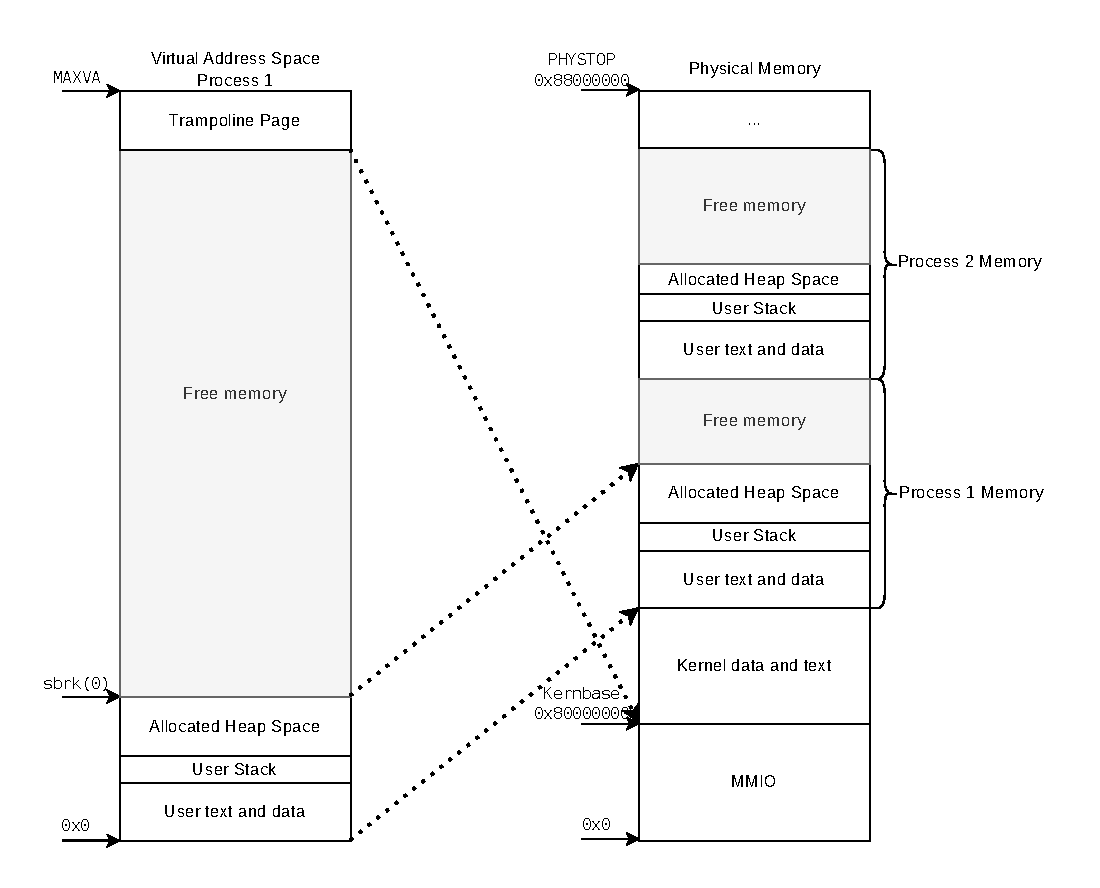
\includegraphics[]{figures/simple_mapping.pdf}

    \caption[Simple Mapping Scheme]{Simple Mapping Scheme}
    \label{fig:theory:simplemapping}
\end{figure*}